\documentclass[crop=false]{standalone}

\usepackage[subpreambles=false]{standalone}
\usepackage{import}
\usepackage{graphicx}
\usepackage{subcaption}
\usepackage{tikz}

\begin{document}

\begin{figure}
  \centering
  % \hspace*{-0.08\linewidth}
     \begin{subfigure}[b]{0.2278\textwidth}
  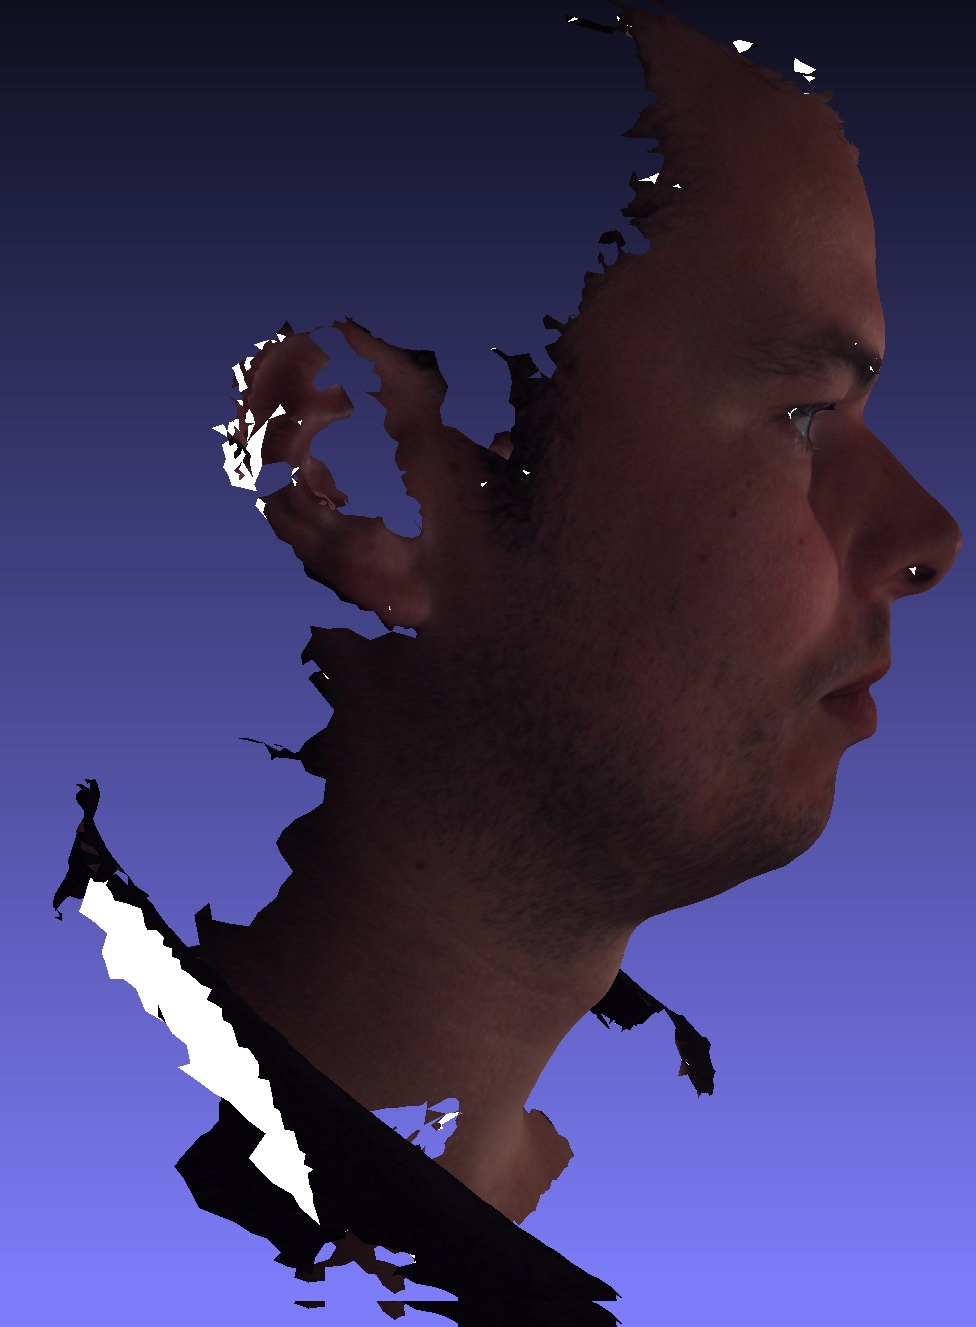
\includegraphics[width=\textwidth]{thesis/results/import/imgs/Untitled6.jpg}
  \caption{}
  \label{fig:1}
  \end{subfigure}
  \begin{subfigure}[b]{0.2282\textwidth}
   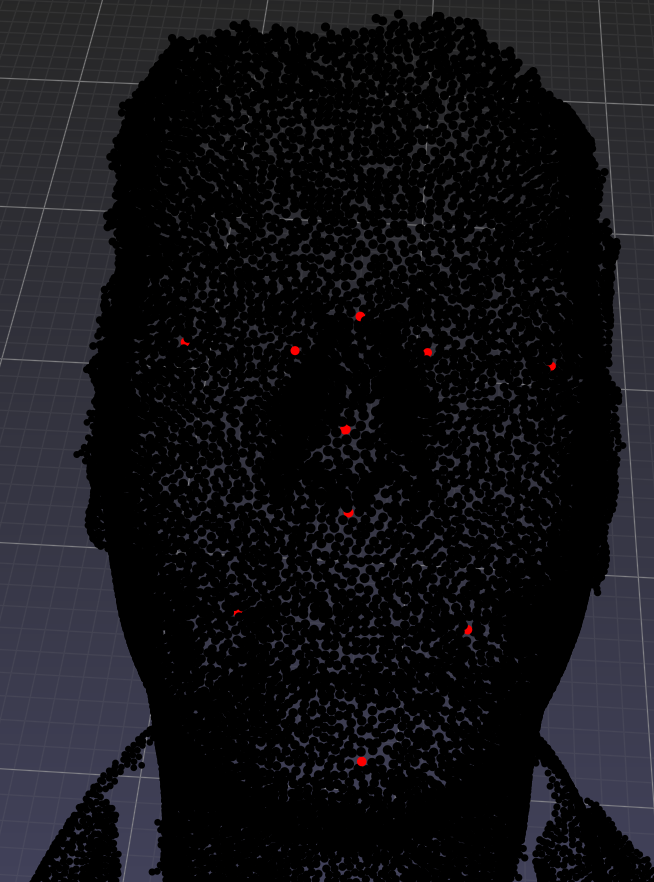
\includegraphics[width=\textwidth]{thesis/results/import/imgs/3.png}
   \caption{}
   \label{fig:2}
   \end{subfigure}
  %\vspace*{-0.06\linewidth}
  \caption{\textbf{Radboudumc prediction example.} \small (a) Side profile of the original mesh. The photo was captured by two cameras, capturing only the face. The head is oriented differently to the pose normalized samples in the training set. The lower mesh quality is also visible in the texture, demonstrated as white spots for faulty textures. (b) Frontal profile of the same subject showing predictions. At first glance, the predictions look seemingly accurate. Quantitative results on Headspace annotations indicate however, that the model trained on HKS is more inaccurate with a mean error over 5mm. 
    
   }
   \label{fig:pred_umc_datax} 
  
\end{figure}

\end{document}